\chapter{Resultados e Discussão}
\label{ch:5_ResultadosDiscucao}
Nesse capítulo são apresentados os resultados obtidos pelos algoritmos e operadores propostos no Capítulo 3. Conforme mencionado no capítulo anterior, os testes foram estruturados em duas etapas, os resultados da primeira etapa são apresentados na Seção \ref{ch:5_Etapa1} enquanto que na Seção \ref{ch:5_Etapa2} são apresentados os resultados da segunda etapa. A seguir um resumo das siglas dos algoritmos utilizados durante os experimentos realizados:

\begin{itemize}
    \item \textbf{$AG^{RPC-1}$}: AG de Regime Permanente com a configuração dada na Tabela \ref{table:con01}
    \item \textbf{$AG^{GC-1}$}: AG Geracional com a configuração dada na Tabela \ref{table:con01}
    \item \textbf{$AG^{RPC-2}$}: AG de Regime Permanente com configuração dada na Tabela \ref{table:con02}
    \item \textbf{$AG^{GC-2}$}: AG Geracional com configuração dada na Tabela \ref{table:con02}
    \item \textbf{$AG^{RPC-3}$}: AG de Regime Permanente com a configuração dada na Tabela \ref{table:con03}
    \item \textbf{$AG^{GC-3}$}: AG Geracional com a configuração dada na Tabela \ref{table:con03}

    \item \textbf{$AG^{RPM}$}: AG de Regime Permanente Modificado com a configuração dada na Tabela \ref{table:con04}
    \item \textbf{$AG^{CO-{100}}$}: AG de Regime Permanente com o Operador de Contagem de Ocorrências com a configuração dada na Tabela \ref{table:con05}
    \item \textbf{$AG^{CO-{50}}$}: AG de Regime Permanente com o Operador de Contagem de Ocorrências com a configuração dada na Tabela \ref{table:con05}

    \item \textbf{$AG^{BL-1}$}: AG de Regime Permanente Modificado com a primeira versão da Busca Local, configuração dada na Tabela \ref{table:con06}
    \item \textbf{$AG^{BL-2}$}: AG de Regime Permanente Modificado com a segunda versão da Busca Local, configuração dada na Tabela \ref{table:con07}

    \item \textbf{$AG^{RPM-730}$}: AG de Regime Permanente Modificado realizando 730 avaliações da função objetivo.
    \item \textbf{$CMOST^{500}$}: $CMOST$ realizando 500 avaliações da função objetivo.
    \item \textbf{$CMOST^{730}$}: $CMOST$ realizando 730 avaliações da função objetivo.
    \item \textbf{$BA$}: Busca Aleatória
\end{itemize}

\section{Etapa 1 – Sem Busca Local}
\label{ch:5_Etapa1}
A Tabela \ref{tab:results1_1} apresenta os resultados obtidos pela execução das versões clássicas do algoritmo genético durante a primeira etapa. Nessa tabela são apresentados o melhor VPL obtido em cada uma das dez execuções das versões do AG. Além disso também são apresentados o VPL médio, o desvio padrão e o tempo médio que cada algoritmo levou para atingir o critério de parada (realizar as 500 avaliações da função objetivo). A Tabela \ref{tab:results1_2} apresenta os mesmo resultados para a execuçao das versões modificadas do algortimo genético, bem como a Busca Aleatória (BA) e o CMOST realizando 500 avaliações da função objetivo ($CMOST^{500}$).

\begin{table}[H]
\centering
\caption{Resultados obtidos pela execução das versões clássicas do Algoritmo Genégico Geracional e de Regime Permanente}
\label{tab:results1_1}
\begin{tabular}{|c|c|c|c|c|c|c|}
\hline
\textbf{Execução} & $AG^{RPC-1}$ & $AG^{GC-1}$ & $AG^{RPC-2}$ & $AG^{GC-2}$ & $AG^{RPC-3}$ & $AG^{GC-3}$ \\ \hline
\textbf{1} & 5,49E+08 & 6,55E+08 & 8,21E+08 & 6,44E+08 & 9,68E+08 & 8,59E+08 \\ \hline
\textbf{2} & 4,82E+08 & 5,63E+08 & 7,92E+08 & 5,92E+08 & 9,20E+08 & 8,20E+08 \\ \hline
\textbf{3} & 6,17E+08 & 7,71E+08 & 8,69E+08 & 5,98E+08 & 9,69E+08 & 8,87E+08 \\ \hline
\textbf{4} & 7,19E+08 & 5,24E+08 & 7,15E+08 & 9,22E+08 & 8,85E+08 & 9,13E+08 \\ \hline
\textbf{5} & 5,14E+08 & 5,50E+08 & 7,56E+08 & 6,47E+08 & 9,72E+08 & 8,65E+08 \\ \hline
\textbf{6} & 7,47E+08 & 8,27E+08 & 6,87E+08 & 8,71E+08 & 9,42E+08 & 8,39E+08 \\ \hline
\textbf{7} & 5,96E+08 & 5,83E+08 & 8,50E+08 & 7,01E+08 & 1,01E+09 & 8,94E+08 \\ \hline
\textbf{8} & 7,19E+08 & 6,67E+08 & 7,02E+08 & 6,52E+08 & 1,05E+09 & 8,29E+08 \\ \hline
\textbf{9} & 6,09E+08 & 6,73E+08 & 7,72E+08 & 7,24E+08 & 9,82E+08 & 8,37E+08 \\ \hline
\textbf{10} & 6,41E+08 & 6,23E+08 & 8,49E+08 & 6,38E+08 & 1,01E+09 & 8,87E+08 \\ \hline

\textbf{Média} & 6,19E+08 & 6,43E+08 & 7,81E+08 & 6,99E+08 & 9,71E+08 & 8,63E+08 \\ \hline
\textbf{Desvio Padrão} & 8,96E+07 & 9,72E+07 & 6,58E+07 & 1,12E+08 & 4,74E+07 & 3,14E+07 \\ \hline
\textbf{Tempo Médio} & 02:39 & 02:36 & 02:34 & 02:31 & 02:44 & 02:10 \\ \hline
\end{tabular}
\end{table}

\begin{table}[H]
\centering
\caption{Resultados obtidos pela execução das versões modificadas do AG, da Busca Aleatória (BA) e do CMOST}
\label{tab:results1_2}
\begin{tabular}{|c|c|c|c|c|c|}
\hline
\textbf{Execução} & $AG^{RPM}$ &	$AG^{CO-{100}}$ & $AG^{CO-{50}}$ & $BA$ & $CMOST^{500}$ \\ \hline
\textbf{1}  & 1,19E+09 & 1,07E+09 & 1,21E+09	 & 8,54E+08	 & 1,54E+09 \\ \hline
\textbf{2} & 1,21E+09 & 1,22E+09 & 1,18E+09	 & 7,06E+08	 & 1,67E+09 \\ \hline
\textbf{3}  & 1,19E+09 & 1,06E+09 & 1,09E+09	 & 7,63E+08	 & 1,40E+09 \\ \hline
\textbf{4}  & 1,22E+09 & 1,10E+09 & 1,11E+09	 & 8,36E+08	 & 1,52E+09 \\ \hline
\textbf{5}  & 1,23E+09 & 1,01E+09 & 1,19E+09	 & 8,36E+08	 & 1,51E+09 \\ \hline
\textbf{6}  & 1,19E+09 & 1,01E+09 & 1,12E+09	 & 8,76E+08	 & 1,62E+09 \\ \hline
\textbf{7}  & 1,11E+09 & 1,06E+09 & 1,11E+09	 & 8,49E+08	 & 1,55E+09 \\ \hline
\textbf{8}  & 1,11E+09 & 1,04E+09 & 1,20E+09	 & 7,76E+08	 & 1,67E+09 \\ \hline
\textbf{9}  & 1,13E+09 & 1,02E+09 & 1,18E+09	 & 8,14E+08	 & 1,57E+09 \\ \hline
\textbf{10}  & 1,22E+09 & 1,13E+09 & 1,07E+09	 & 8,24E+08	 & 1,66E+09 \\ \hline

\textbf{Média}  & 1,18E+09 & 1,07E+09 & 1,15E+09   & 8,14E+08 & 1,57E+09 \\ \hline
\textbf{Desvio Padrão}  & 4,60E+07 & 6,50E+07 & 5,10E+07   & 5,11E+07 & 8,62E+07 \\ \hline
\textbf{Tempo Médio}   & 02:45 & 05:12 & 04:16 & 02:53 & 07:15 \\ \hline

\end{tabular}
\end{table}

As próximas seções apresentam, com mais detalhes, cada um dos experimentos realizados e os resultados obtidos.

\subsection{Experimento 1}
\label{ch:5_Experimento1}
Nesse primeiro experimento foram utilizadas as versões clássicas do Algoritmo Genético Geracional ($AG^{GC-1}$) e do Algoritmo Genético de Regime Permanente ($AG^{RPC-1}$), bem como versões clássicas dos operadores de seleção, recombinação e mutação. Ao observar os resultados obtidos pelo $AG^{GC-1}$ e o $AG^{RPC-1}$ é possível notar que o desempenho das versões clássicas do AG, com os operadores clássicos, foi aquém do esperado. Os AGs com as configurações propostas não foram capazes de obter soluções superiores às da busca aleatória.  A BA conseguiu obter soluções com VPL 32\% melhor às do $AG^{RPC-1}$ e 27\% melhor que as do $AG^{GC-1}$, uma diferença considerável. Ao comparar os AGs com o $CMOST^{500}$ a diferença foi ainda maior. O VPL médio das soluções obtidas pelo $CMOST^{500}$ é cerca de 2,5 vezes superior aos resultados obtidos pelos AGs.

As Figuras \ref{fig:graph1_1} e \ref{fig:graph1_2}, apresentam a evolução da melhor solução, da pior solução e da média da população durante a 4ª execução do $AG^{RPC-1}$ e da 1ª execução do $AG^{GC-1}$. Os gráficos para as demais execuções são apresentados no Apêndice A.

Pelas figuras \ref{fig:graph1_1} e \ref{fig:graph1_2}, é possível notar a forma como a estratégia de busca adotada por cada AG impacta na qualidade dos indivíduos da população no decorrer das gerações. Enquanto no $AG^{RPC-1}$ o \textit{fitness} médio da população ou se mantém constante ou apresenta melhoria no decorrer das gerações, com o $AG^{GC-1}$ há sempre uma grande variação do \textit{fitness} médio. Isso é um reflexo da abordagem para a manutenção da população adotada por cada versão do AG. Na abordagem geracional do algoritmo genético, utilizada pelo $AG^{GC-1}$, uma nova população é gerada a cada iteração, isso permite que soluções ruins façam parte da população, por isso essa versão do AG apresenta grande variação no \textit{fitness} médio durante as iterações. O mesmo não ocorre com a abordagem de regime permanente: como só é gerada uma solução por iteração e essa solução só é incluída na população caso apresente um VPL melhor que algum indivíduo, observa-se uma evolução mais consistente da média do VPL da população.

\begin{figure}[htb]
    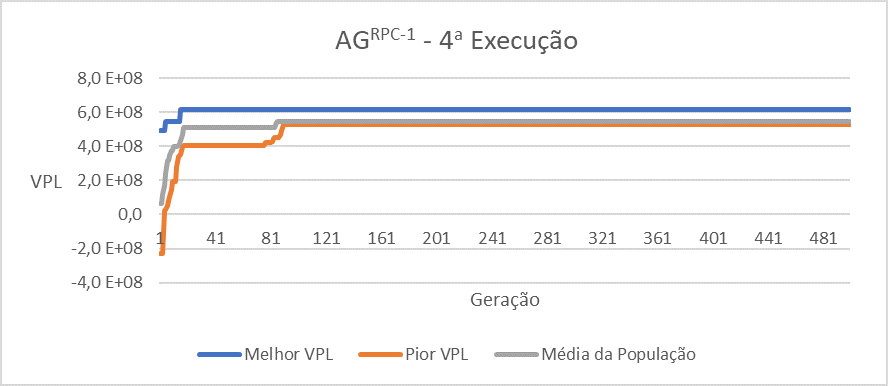
\includegraphics[scale=1]{6}
    \caption{Evoluçao do VPL para a quarta execução da versão clássica Algoritmo Genético de Regime Permanente com operadores de busca clássicos.}
    \label{fig:graph1_1}
\end{figure}

\begin{figure}[htb]
    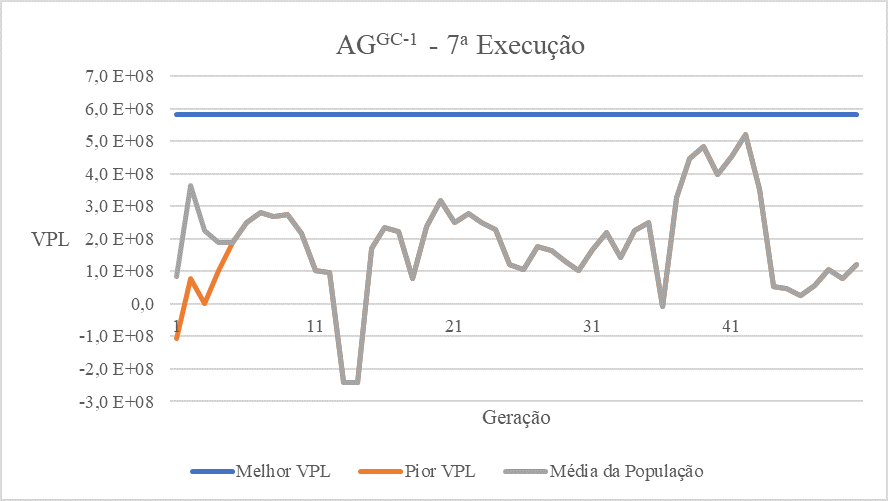
\includegraphics[scale=1]{7}
    \caption{Evoluçao do VPL para a primeira execução da versão clássica Algoritmo Genético Geracional com operadores de busca clássicos.}
    \label{fig:graph1_2}
\end{figure}

Ainda é possível notar, pelas figuras \ref{fig:graph1_1} e \ref{fig:graph1_2}, que em ambos os AGs a melhor solução foi encontrada no início do processo de busca (gerações iniciais). É provável que os AGs, com os operadores e parâmetros utilizados nesse experimento, não tenham sido capazes de explorar de forma satisfatória o espaço de busca. Essa ideia é reforçada ao observar evolução do VPL médio e do pior VPL obtido pelo $AG^{RPC-1}$, durante várias gerações tanto o VPL médio quanto o pior VPL da população mantiveram-se os mesmos. Diante disso, é possível inferir que a população foi perdendo a diversidade e que as soluções geradas não foram suficientemente boas para serem incluídas na população.

Para verificar o quão significativo foram os resultados obtidos nesse experimento, foi aplicado o teste de Mann-Whitney-Wilcoxon, considerando-se um limiar de 5\%. Os resultados dos testes são apresentados na Tabela \ref{tab:mw1_1}.

\begin{table}[H]
\centering
\caption{Resultados obtidos (\textit{p-value}) ao aplicar o teste não-paramétrico de Mann-Whitney-Wilcoxon}
\label{tab:mw1_1}
\begin{tabular}{|c|c|c|}
\hline
\multicolumn{2}{|c|}{Algoritmos Comparados} & Resultados \\ \hline
$AG^{RPC-1}$ &	$AG^{GC-1}$ & 79,590\% \\ \hline
$AG^{RPC-1}$ & $CMOST^{500}$ & 0,018\% \\ \hline
$AG^{RPC-1}$ & BA & 0,032\% \\ \hline
$AG^{GC-1}$ & $CMOST^{500}$ & 0,018\% \\ \hline
$AG^{GC-1}$ & BA & 0,049\% \\ \hline

\end{tabular}
\end{table}

Pelos resultados reportados pela Tabela \ref{tab:mw1_1}, podemos concluir que, além dos resultados inferiores aos obtidos pela BA e CMOST, não há diferença entre utilizar o AG Geracional ($AG^{GC-1}$) ou o AG de Regime Permanente ($AG^{RPC-1}$) com os parâmetros e operadores adotados nesse primeiro experimento. No entanto, a diferença entre os resultados dos AG e o $CMOST^{500}$ e a BA se mostraram  significativas.

\subsection{Experimento 2}
\label{ch:5_Experimento2}
Nesse experimento, a principal mudança realizada foi a alteração do operador de recombinação dos AGs. No lugar da Recombinação Uniforme optou-se por um operador novo, conforme descrito na Seção \ref{sec:3_OperadorRecombinacao}. Tal operador posiciona os poços da nova solução dentro da região delimitada pelas coordenadas dos poços de duas soluções previamente selecionadas (pais). Novamente, foram utilizadas tanto a versão clássica do Algoritmo Genético Geracional ($AG^{GC-2}$) quanto o Algoritmo Genético de Regime permanente ($AG^{RPC-2}$).

Como é possível perceber à partir dos resultados apresentados na Tabela \ref{tab:results1_1}, tanto o $AG^{RPC-2}$ quanto o $AG^{GC-2}$ apresentaram desempenho melhor que os obtidos pelos AGs do Experimento 1. A mudança do operador de recombinação se mostrou satisfatória, principalmente para a abordagem de regime permanente. Em média, os resultados do $AGR^{RPC-2}$ foram 23\% melhores que os obtidos pelo $AG^{RPC-1}$. A versão geracional do AG utilizada nesse experimento também apresentou melhoras em relação ao experimento anterior, mas os resultados obtidos pelo $AG^{GC-2}$ foram, em média, apenas 9\% melhores.

No entanto, apesar das melhorias observadas, ambas as versões do AG novamente tiveram um desempenho aquém da BA e, principalmente, do $CMOST^{500}$. Apesar dos AGs levarem cerca 36\% do tempo gasto pelo $CMOST^{500}$ para concluírem as 500 avaliações, o VPL médio obtido pelo $CMOST^{500}$ ainda chega a ser o dobro do VPL médio obtido pelos AGs. Com as configurações adotadas nesse experimento, os AGs ainda não foram capazes de explorar de forma adequada o espaço de busca para obter soluções de boa qualidade. 

Ao aplicar o teste de Mann-Whitney-Wilcoxon entre o $AG^{RPC-2}$ e o $AG^{GC-2}$, a diferença entre os resultados se mostraram mais significativas obtendo o valor de 5,24\%. Apesar do resultado ser acima do limiar de 5\%, aqui já é possível observar há uma diferença entre as abordagens geracional e de regime permanente. A Tabela \ref{tab:mw2_1} reporta o resultado do teste ao comparar os resultados do $AG^{RPC-2}$ com os AGs do Experimento 1, o CMOST e a BA. 

\begin{table}[H]
\centering
\caption{Resultados do teste de Mann-Whitney-Wilcoxon para comparar os resultados do $AG^{RPC-2}$, os AGs do Experimento 1, o $CMOST^{500}$ e a BA}
\label{tab:mw2_1}
\begin{tabular}{|c|c|c|}
\hline
\multicolumn{2}{|c|}{Algoritmos Comparados} & Resultados \\ \hline
$AG^{RPC-2}$ & $AG^{RPC-1}$ & 0,68\% \\ \hline
$AG^{RPC-2}$ & $AG^{GC-1}$ & 0,21\% \\ \hline
$AG^{RPC-2}$ & $CMOST^{500}$ & 0,02\% \\ \hline
$AG^{RPC-2}$ & BA & 27,99\% \\ \hline
\end{tabular}
\end{table}

Além do desempenho melhor do $AG^{RPC-2}$ em relação aos AGs do Experimento 1, a diferença entre o resultado obtido aqui e os obtidos anteriormente também se mostraram significativos segundo o teste realizado considerando um limiar de 5\%. O mesmo vale para o $CMOST^{500}$. Em relação à BA, apesar de ter uma média ainda melhor que o $AG^{RPC-2}$, não há uma diferença entre usar o AG e a BA, já que o resultado do teste ultrapassa o limiar de 5\%. Em relação ao $AG^{GC-2}$, os resultados do teste de Mann-Whitney-Wilcoxon indicam que os valores de VPL encontrados não são semelhantes aos obtidos pelo $AG^{RPC-2}$. Segundo os resultados obtidos, não há diferenças estisticamente significativas entre o AG Geracional desse experimento e os AGs do experimento anterior. No entanto, ao se comparar o $AG^{GC-2}$ com o $CMOST^{500}$ e a BA, o teste mostrou que há uma diferença significativa entre os resultados obtidos pelo $AG^{GC-2}$ e os dessas ferramentas. A Tabela \ref{tab:mw2_2} apresenta os resultados do teste de Mann-Whitney-Wilcoxon aplicado ao $AG^{GC-2}$.

\begin{table}[htb]
\centering
\caption{Resultados do teste de Mann-Whitney-Wilcoxon para comparar os resultados do $AG^{GC-2}$, os AGs do Experimento 1, o $CMOST^{500}$ e a BA.}
\label{tab:mw2_2}
\begin{tabular}{|c|c|c|}
\hline
\multicolumn{2}{|c|}{Algoritmos Comparados} & Resultados \\ \hline
$AG^{GC-2}$ & $AG^{RPC-1}$ & 27,99\% \\ \hline
$AG^{GC-2}$ & $AG^{GC-1}$ & 48,13\% \\ \hline
$AG^{GC-2}$ & $CMOST^{500}$ & 0,02\% \\ \hline
$AG^{GC-2}$ & BA & 2,32\% \\ \hline

\end{tabular}
\end{table}

As figuras \ref{fig:graph2_1} e \ref{fig:graph2_2} apresentam os gráficos da evolução do melhor VPL, do pior VPL e do valor médio do VPL da população ao longo da $10^a$ execução do $AG^{RPC-2}$ e do $AG^{GC-2}$, respectivamente. Para as demais execuções, os gráficos são apresentados no Apêndice B.  Como é possível notar na Figura \ref{fig:graph2_1}, o $AG^{RPC-2}$ ainda apresenta o mesmo problema observado no AG de Regime Permanente do experimento anterior, mesmo que em intensidade menor: apesar de alguns saltos de melhorias do decorrer do processo de busca, durante várias gerações tanto o VPL médio quanto o pior VPL da população do $AG^{RPC-2}$ mantiveram-se os mesmos. Diante disso, é possível reafirmar que, mesmo com a melhorias, essa versão do AG ainda gera uma quantidade considerável de soluções que não são suficientemente boas para serem incluídas na população, o que prejudicou o desempenho da busca do AG. Quando ao $AG^{GC-2}$, é possível notar, pela Figura \ref{fig:graph2_2}, a grande variação de qualidade das soluções do decorrer das gerações. 

Como dito anteriormente, esse é um reflexo da abordagem escolhida para a manutenção da população.

\begin{figure}[H]
\centering
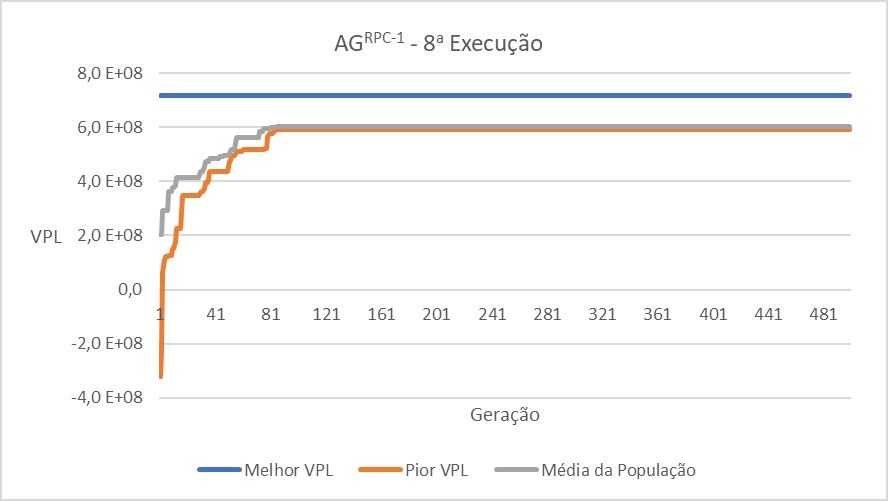
\includegraphics[scale=1]{8}
\caption{Evolução do VPL obtido pela melhor solução, pela pior solução e a média da população obtida através da $10^a$ execução do $AG^{RPC-2}$.}
\label{fig:graph2_1}
\end{figure}

\begin{figure}[H]
\centering
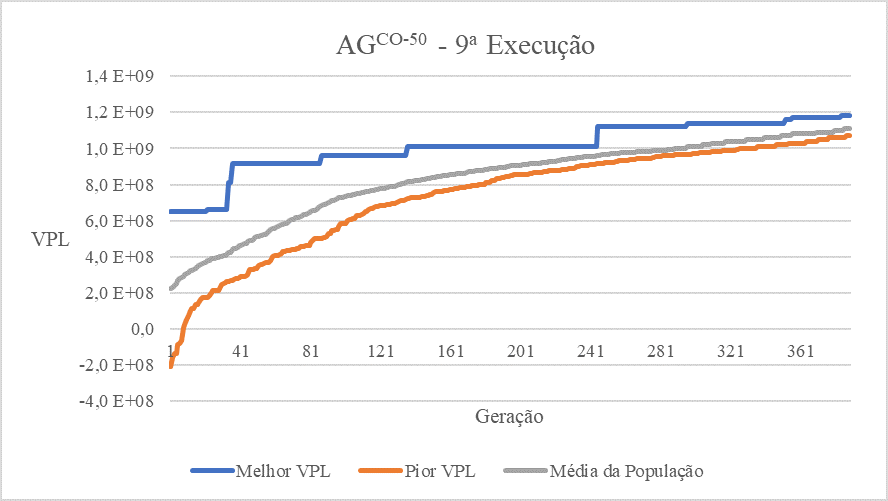
\includegraphics[scale=1]{9}
\caption{Evolução do VPL obtido pela melhor solução, pela pior solução e a média da população obtida através da $10^a$ execução do $AG^{GC-2}$.}
\label{fig:graph2_2}
\end{figure}

\subsection{Experimento 3}
\label{ch:5_Experimento3}
Para o terceiro experimento dessa etapa ainda foram consideradas as versões clássicas dos AGs. Tanto a abordagem de regime permanente ($AG^{RPC-3}$) quanto a geracional ($AG^{GC-3}$) foram mantidas, e o mesmo vale para os operadores de seleção, recombinação e mutação. A principal alteração realizada nesse terceiro experimento se deu em relação aos parâmetros utilizados pelos AGs. Analisando-se os parâmetros dos algoritmos, percebeu-se que um aumento no número de indivíduos da população inicial poderia distribuir melhor as soluções iniciais. Sendo assim, conforme apresentado no Capítulo 4.3, esse parâmetro passou de 10 para 100 indivíduos.

Ao observar os resultados reportados na Tabela \ref{tab:results1_1} nota-se uma melhora no VPL médio obtido pelos AGs utilizando os parâmetros propostos nesse terceiro experimento em relação ao VPL médio obtido anteriormente. Dessa vez os AGs conseguiram um VPL médio cerca de 24\% melhor que o apresentado pelos AGs do Experimento 2. Quando comparados com a BA (Tabela \ref{tab:results1_2}), a melhora fica em cerca de 19\% para o $AG^{RPC-3}$ e de 6\% para o $AG^{GC-3}$. No entanto, apesar dos resultados melhores, as duas versões do AG novamente não conseguiram superar as soluções obtidas pelo $CMOST^{500}$. Ainda assim, é importante destacar que os AGs desse experimento completam as 500 avaliações com cerca de 37\% do tempo que o $CMOST^{500}$ (Tabela \ref{tab:results1_2}) precisou para concluir a mesma quantidade de avaliações.

Ao aplicar o teste de Mann-Whitney-Wilcoxon com limiar de 5\%, observou-se que a diferença entre os resultados obtidos pelos AGs desse experimento é estatisticamente significativa (0,013\%). Assim como foi feito no experimento anteriores, os resultados obtidos aqui foram comparados com os resultados obtidos pelo $CMOST^{500}$ e a BA. Além disso os AGs desse experimento também foram comparados com os AGs do Experimento 2. A Tabela \ref{tab:mw3_1} apresenta os resultados do teste estatístico obtidos ao comparar o resultado do $AG^{RPC-3}$ com os algoritmos já citados.

\begin{table}[H]
\centering
\caption{Resultados do teste de Mann-Whitney-Wilcoxon para comparar os resultados do $AG^{RPC-3}$, os AGs do Experimento 2, o $CMOST^{500}$ e a BA.}
\label{tab:mw3_1}
\begin{tabular}{|c|c|c|}
\hline
\multicolumn{2}{|c|}{Algoritmos Comparados} & Resultados \\ \hline
$AG^{RPC-3}$ & $AG^{RPC-2}$ & 0,0011\% \\ \hline
$AG^{RPC-3}$ & $AG^{GC-2}$ & 0,0043\% \\ \hline
$AG^{RPC-3}$ & $CMOST^{500}$ & 0,0182\% \\ \hline
$AG^{RPC-3}$ & BA & 0,0011\% \\ \hline

\end{tabular}
\end{table}

Como é possível notar na Tabela \ref{tab:mw3_1}, a diferença entre os resultados obtidos pelo $AG^{RPC-3}$ e os AGs do Experimento 2 é estatisticamente significativa, e o mesmo pode ser dito em relação à comparação do $AG^{RPC-3}$ com o $CMOST^{500}$ e a BA. O $AG^{GC-3}$ também obteve um resultado semelhante, conforme pode ser observado pela Tabela \ref{tab:mw3_2}.

\begin{table}[H]
\centering
\caption{Resultados do teste de Mann-Whitney-Wilcoxon para comparar os resultados do $AG^{GC-3}$, os AGs do Experimento 2, o $CMOST^{500}$ e a BA}
\label{tab:mw3_2}
\begin{tabular}{|c|c|c|}
\hline
\multicolumn{2}{|c|}{Algoritmos Comparados} & Resultados \\ \hline
$AG^{GC-3}$ & $AG^{RPC-2}$ & 0,6841\% \\ \hline
$AG^{GC-3}$ & $AG^{GC-2}$ & 0,8931\% \\ \hline
$AG^{GC-3}$ & $CMOST^{500}$ & 0,0182\% \\ \hline
$AG^{GC-3}$ & BA & 1,8540\% \\ \hline

\end{tabular}
\end{table}

As figuras \ref{fig:graph3_1} e \ref{fig:graph3_2} apresentam os gráficos da evolução do melhor VPL, do pior VPL e o valor médio do VPL da população durante a $5^a$ execução do $AG^{RPC-3}$ e do $AG^{GC-3}$, respectivamente. Os gráficos para as demais execuções são apresentados no Apêndice C. 

\begin{figure}[H]
\centering
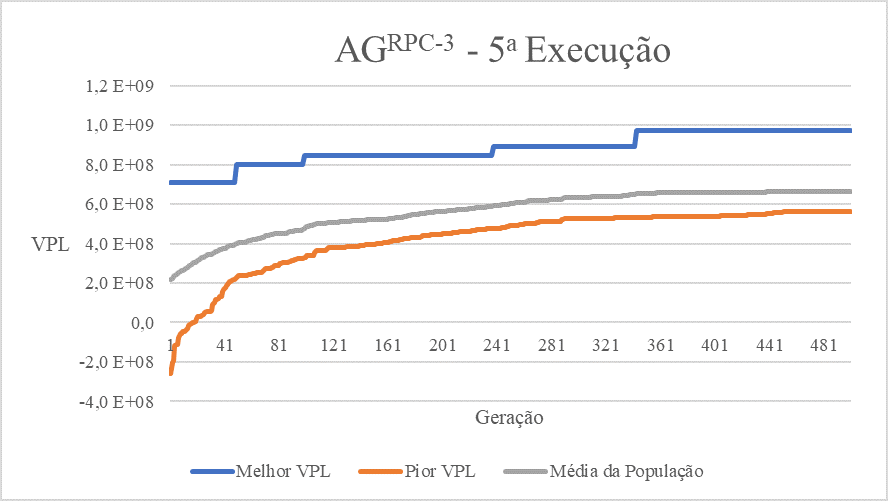
\includegraphics[scale=1]{10}
\caption{ Evolução do VPL obtido pela melhor solução, pela pior solução e a média da população obtida na $5^a$ execução do $AG^{RPC-3}$}
\label{fig:graph3_1}
\end{figure}

\begin{figure}[H]
\centering
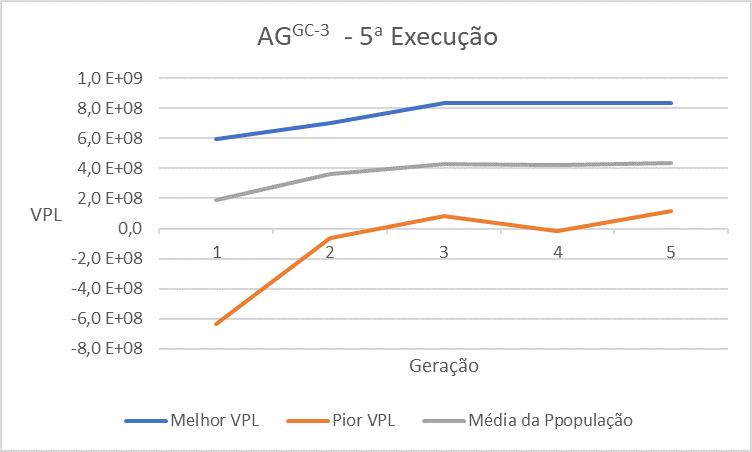
\includegraphics[scale=1]{11}
\caption{Evolução do VPL obtido pela melhor solução, pela pior solução e a média da população obtida na $5^a$ execução do $AG^{GC-3}$}
\label{fig:graph3_2}
\end{figure}

Ao comparar evolução do VPL médio da população e do pior VPL do $AG^{RPC-3}$ (Figura \ref{fig:graph3_1}) e comparar com a evolução da população do $AG^{RPC-2}$ (Figura \ref{fig:graph2_1}), percebe-se que a população do $AG^{RPC-3}$ raramente passa alguma geração sem apresentar uma melhora no \textit{fitness} médio da população ou no pior \textit{fitness}, ao contrário do que acontece com o $AG^{RPC-2}$. Quanto à versão geracional do algoritmo, o $AG^{GC-3}$, nota-se que a quantidade de gerações foi consideravelmente reduzida, uma vez que, ao considerar-se uma população com 100 indivíduos, a cada geração, 100 novas avaliações da função objetivo são realizadas, sendo assim são necessários somente 5 gerações dessa versão do AG para atingir o limite de 500 avaliações. Apesar disso, o $AG^{GC-3}$ ainda apresentou um resultado melhor que o das duas versões de AG do experimento anterior. Sendo assim, pode-se afirmar que o aumento da população foi vantajoso para as duas versões do AG, uma vez que esses algoritmos utilizam a população como um repertório para explorar o espaço de busca. Com um repertório maior, a exploração tornou-se mais eficiente.

\subsection{Experimento 4}
\label{ch:5_Experimento4}
A partir dos resultados dos três primeiros experimentos, é possível notar que o AG de Regime Permanente levou ao melhor desempenho até então. Diante disso, essa variação do algoritmo genético foi tomada como base para as alterações da segunda versão do AG apresentada na Seção \ref{sec:3_SegundaVersao}.  Nesse quarto experimento, a tentativa de melhoria dessa versão do algoritmo se deu através da introdução de um novo operador de mutação que utiliza alterações aleatória nos poços da solução com base no IEP de cada poço: a amplitude da alteração realizada em um dado poço é inversamente proporcional ao IEP desse poço, conforme apresentado na Seção \ref{sec:3_OperadorMutacao}. Os demais operadores e parâmetros foram mantidos.

Utilizar o IEP como parâmetro para manipulação dos poços da Estratégia de Produção trouxe grandes melhorias ao desempenho do algoritmo. Como é possível observar nos dados apresentados na Tabela \ref{tab:results1_2} (coluna $AG^{RPM}$), em todas as execuções o VPL obtido foi superior aos resultados obtidos pelos AGs dos experimentos anteriores. A modificação do operador de mutação levou a um ganho de 21,5\% no VPL médio do algoritmo em relação ao experimento anterior. Este ganho observado também foi considerado estatisticamente significativo, segundo o teste de Mann-Whitney-Wilcoxon (considerando um limiar de 5\%), comparando o algoritmo desse experimento com os AGs do experimento anterior. A Tabela \ref{tab:mw4_1} apresenta o resultado do teste estatístico.

\begin{table}[H]
\centering
\caption{Resultados do teste de Mann-Whitney-Wilcoxon para comparar os resultados do $AG^{RPM}$, os AGs do Experimento 3, o $CMOST^{500}$ e a BA}
\label{tab:mw4_1}
\begin{tabular}{|c|c|c|}
\hline
\multicolumn{2}{|c|}{Algoritmos Comparados} & Resultados \\ \hline
$AG^{RPM}$ & $AG^{RPC-3}$ & 0,0011\% \\ \hline
$AG^{RPM}$ & $AG^{GC-3}$ & 0,0011\% \\ \hline
$AG^{RPM}$ & $CMOST^{500}$ & 0,0182\% \\ \hline
$AG^{RPM}$ & BA & 0,0011\% \\ \hline


\end{tabular}
\end{table}

No entanto, apesar das melhorias, o algoritmo genético ainda não foi capaz de superar o resultado obtido pelo $CMOST^{500}$. O VPL médio obtido por essa ferramenta ainda é cerca de 33\% superior ao obtido pelo AG desse experimento. Ainda assim, o $AG^{RPM}$ foi capaz de completar as 500 avaliações com um tempo consideravelmente menor, cerca de 38\% do tempo gasto pelo $CMOST^{500}$.

A Figura \ref{fig:graph4_1} apresenta a evolução do VPL da melhor solução, do VPL médio da população e do VPL da pior solução obtidos ao longo da $1^a$ execução dessa versão do algoritmo. É possível notar, pela Figura \ref{fig:graph4_1}, que há evolução do VPL médio da população, basicamente, em todas as iterações, um comportamento semelhante ao observado pelo $AG^{RPC-3}$ no experimento anterior. Vale ressaltar que, para as demais execuções, os gráficos são apresentados no Apêndice D.

\begin{figure}[H]
\centering

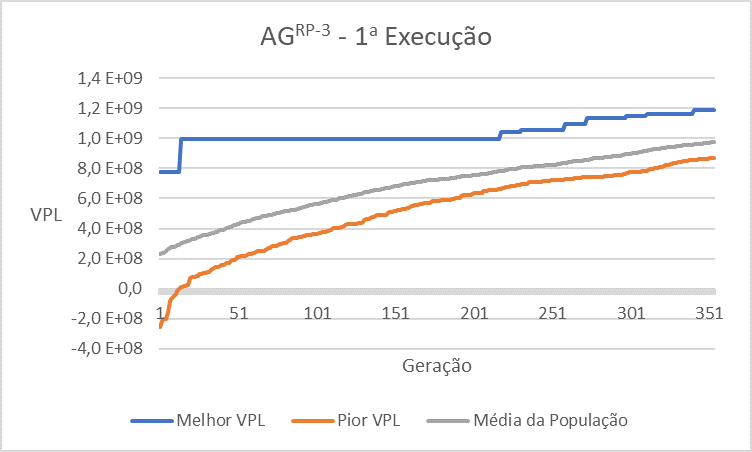
\includegraphics[scale=1]{12}

\caption{Evolução do VPL obtido pela melhor solução, para a pior solução e a média da população obtida na $1^a$ execução do $AG^{RPM}$}
\label{fig:graph4_1}
\end{figure}

\subsection{Experimento 5}
\label{ch:5_Experimento5}
Para o último experimento dessa etapa, foi considerada a terceira versão do algoritmo genético apresentado na Seção \ref{sec:3_TerceiraVersao}, que também segue a abordagem de regime permanente. Para testar o conceito proposto para essa versão do AG, foram utilizados dois tamanhos de população: 100 indivíduos ($AG^{CO-{100}}$) e 50 indivíduos ($AG^{CO-{50}}$). Tal escolha foi feita, nesse experimento, a fim de se observar como o algoritmo se comporta com o operador proposto na Seção \ref{sec:3_ContadorOcorrencias}, uma vez que os valores escolhidos para as soluções que compõem a população inicial servem como ponto de partida para esse operador (cálculo do \textit{score}).

O $AG^{CO-{50}}$ apresentou um VPL médio consideravelmente melhor que o $AG^{CO-{100}}$ (Tabela \ref{tab:results1_2}). É possível intuir que, com uma população menor a distribuição dos valores para cada intervalo definido para as restrições de posicionamento dos poços foi mais equilibrada. No $AG^{CO-{50}}$ posições pouco promissoras para os poços podem ter apresentado maior probabilidade de serem escolhidas pelo operador, gerando soluções não tão promissoras. Observando a evolução da população do $AG^{CO-{50}}$, apresentada na Figura \ref{fig:graph5_2}, percebe-se que a média do VPL da população se aproxima bastante do VPL da melhor solução, mais que o próprio $AG^{CO-{100}}$, cuja evolução é dada na Figura \ref{fig:graph5_1}, e dos AGs dos experimentos anteriores. Isso pode indicar uma perda da diversidade entre os indivíduos da população, o que não é algo desejado para uma boa exploração do espaço de busca. Apesar do ganho de VPL com a população menor nesse AG, há o risco da perda da diversidade da população. Mais uma vez, os gráficos para as demais execuções das duas versões aqui apresentadas encontram-se no Apêndice E.

\begin{figure}[H]
\centering
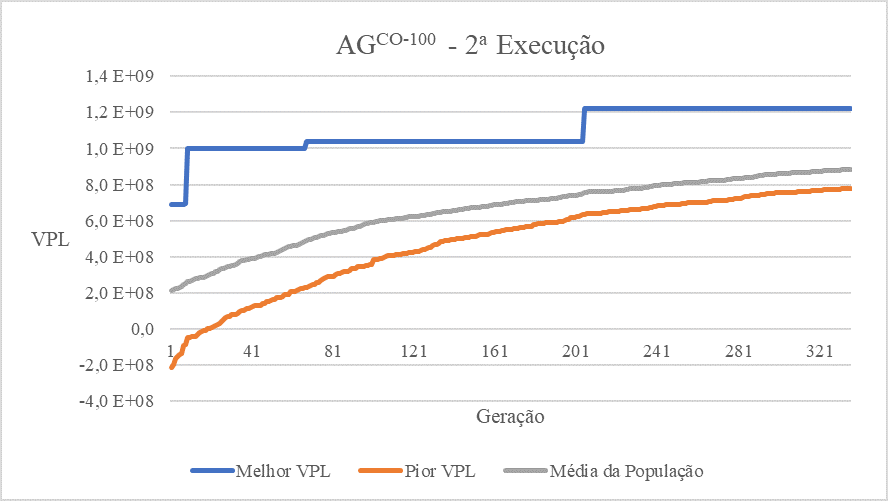
\includegraphics[scale=1]{13}
\caption{Evolução do VPL obtido pela melhor solução, pior solução e a média da população na $2^a$ execução do $AG^{CO-{100}}$}
\label{fig:graph5_1}
\end{figure}

\begin{figure}[H]
\centering
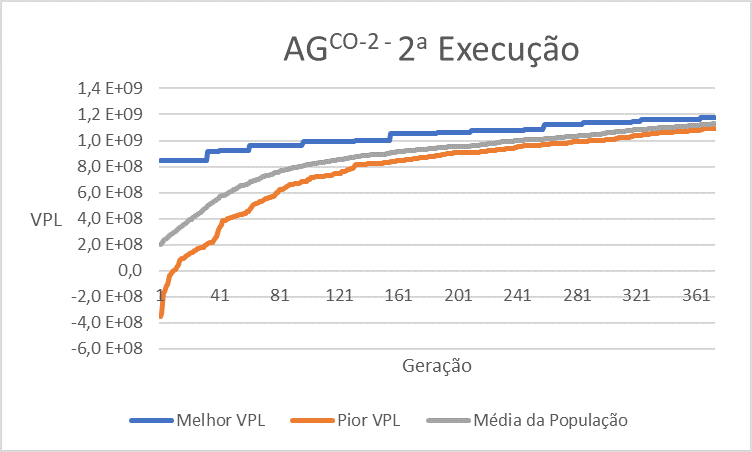
\includegraphics[scale=1]{14}
\caption{Evolução do VPL obtido pela melhor solução, pior solução e a média da população obtida na $2^a$ execução do $AG^{CO-{50}}$}
\label{fig:graph5_2}
\end{figure}

Ao aplicar o teste de Mann-Whitney-Wilcoxon entre o $AG^{CO-{100}}$ e o $AG^{CO-{50}}$, constata-se que a diferença entre os resultados desses AGs é significativa. Mais uma vez utilizando o limiar de 5\%, o teste obteve como resultado 1,40\%.  Tal teste também foi aplicado entre os AGs desse experimento e o $AG^{RPM}$, versão do AG que obteve o melhor resultado até o momento. Os resultados são apresentados na Tabela \ref{tab:mw5_1}.

\begin{table}[H]
\centering
\caption{Resultados do teste de Mann-Whitney-Wilcoxon para comparar os resultados do $AG^{CO-{100}}$ e do $AG^{CO-{50}}$ com o $AG^{RPM}$}
\label{tab:mw5_1}
\begin{tabular}{|c|c|c|}
\hline
\multicolumn{2}{|c|}{Algoritmos Comparados} & Resultados \\ \hline
$AG^{CO-{100}}$ & $AG^{RPM}$ & 0,10\% \\ \hline
$AG^{CO-{50}}$ & $AG^{RPM}$ & 6,40\% \\ \hline

\end{tabular}
\end{table}

Como é possível notar pela Tabela \ref{tab:mw5_1}, apesar do $AG^{CO-{100}}$ ter resultados diferentes e estatisticamente significativos, o $AG^{CO-{50}}$, que apresentou resultados melhores, não possui uma diferença estatisticamente significativa. Sendo assim, optou-se por não levar adiante essa abordagem.

\section{Etapa 2 – Com Busca Local}
\label{ch:5_Etapa2}
Na segunda etapa dos experimentos o foco esteve na exploração das duas versões da busca local descritas na Seção \ref{sec:3_OperadorBuscaLocal}. No total, foram dois experimentos realizados nessa etapa, sendo que em cada um dos experimentos foi utilizada uma das versões do operador de busca local proposto, em conjunto com o AG que obteve o melhor desempenho na etapa anterior, nesse caso o $AG^{RPM}$ do Experimento 4 da Etapa 1. No primeiro experimento dessa segunda etapa foi utilizado com o $AG^{RPM}$ a primeira versão da busca local ($AG^{BL-1}$). No segundo experimento realizado, o AGRPM foi executado com a segunda versão da busca local ($AG^{BL-2}$). Vale ressaltar que os operadores de busca local refinam somente a melhor solução encontrada pelo AG, conforme descrito na Seção \ref{sec:3_OperadorBuscaLocal}.

Apesar da intenção de se comparar os resultados aqui obtidos com os resultados alcançados por $AG^{RPM}$ e  $CMOST^{500}$ na Etapa 1, tal comparação não seria de todo justa. Os AGs dos experimentos realizados nessa etapa precisaram, em média, de um total de 720 avaliações da função objetivo (simulações) para concluir cada execução, 220 avaliações a mais que as utilizadas durante a etapa anterior. Sendo assim, o $AG^{RPM}$ foi executado novamente, mas com um limite de 730 avaliações como critério de parada para que, dessa forma, a comparação fosse justa. O mesmo foi feito para a ferramenta CMOST. Para não haver confusão, o $AG^{RPM}$ executado nessa etapa será referenciado como $AG^{RPM-730}$ e o CMOST como $CMOST^{730}$. 

A Tabela \ref{tab:results2_1} apresenta o melhor VPL obtido por cada uma das dez execuções do $AG^{BL-1}$ e do $AG^{BL-2}$. Além disso, também é apresentado o VPL médio de cada algoritmo, o desvio padrão, o tempo médio, em horas, gasto para cada execução do algoritmo ser concluída e a média de avaliações necessárias para completar a execução dos AGs com busca local. Esses resultados, com exceção da média de avaliações, também são apresentados para $AG^{RPM-730}$ e $CMOST^{730}$.

\begin{table}[H]
\centering
\caption{Resultados obtidos pela execução dos AGs com Busca Local, do melhor AG da Etapa 1 ($AG^{RPM}$) e do CMOST, ambos com 730 avaliações.}
\label{tab:results2_1}
\begin{tabular}{|c|c|c|c|c|}
\hline
Execução & $AG^{BL-1}$ & $AG^{BL-2}$ & $AG^{RPM-730}$ & $CMOST^{730}$ \\ \hline
1 & 1,47E+09 & 1,53E+09 & 1,46E+09 & 1,75E+09 \\ \hline
2 & 1,54E+09 & 1,57E+09 & 1,28E+09 & 1,70E+09 \\ \hline
3 & 1,44E+09 & 1,53E+09	& 1,26E+09 & 1,87E+09 \\ \hline
4 & 1,53E+09 & 1,52E+09 & 1,32E+09 & 1,61E+09 \\ \hline
5 & 1,47E+09 & 1,60E+09 & 1,35E+09 & 1,75E+09 \\ \hline
6 & 1,47E+09 & 1,56E+09 & 1,40E+09 & 1,59E+09 \\ \hline
7 & 1,52E+09 & 1,53E+09 & 1,37E+09 & 1,66E+09 \\ \hline
8 & 1,55E+09 & 1,57E+09 & 1,23E+09 & 1,77E+09 \\ \hline
9 & 1,58E+09 & 1,48E+09 & 1,31E+09 & 1,68E+09 \\ \hline
10 & 1,60E+09 & 1,46E+09 & 1,43E+09 & 1,74E+09\\ \hline
Média & 1,52E+09 & 1,53E+09 & 1,34E+09 & 1,71E+09\\ \hline
Desvio Padrão & 5,28E+07 & 4,08E+07 & 7,39E+07 & 8,11E+07\\ \hline
Tempo Médio & 04:18 & 06:17 & 03:49 & 22:50\\ \hline
Média do Avaliações & 720 & 680	 & - & --\\ \hline

\end{tabular}
\end{table}

As próximas seções discutem, com mais detalhes, os experimentos realizados e os resultados obtidos. 


\subsection{Experimento 1}
\label{ch:5_Experimento6}
Como descrito na Seção \ref{sec:4_MetodologiaExperimental}, nesse experimento o AG foi executado em conjunto com a primeira versão da busca local proposta no Capítulo 3.5. Esse operador de busca local procura, para cada poço da estratégia de produção, verificar uma nova posição em sua vizinhança que leve a ganhos do VPL. Essa busca é realizada até que não haja novas posições que levem a ganhos.

A adição do operador de busca local ao algoritmo genético levou a um ganho de cerca de 29\% do VPL médio quando comparado com o $AG^{RPM}$, executado no Experimento 4 da etapa anterior. O AG com a busca local conseguiu um VPL médio de 1,52E+09 enquanto o $AG^{RPM}$ da Etapa 1 conseguiu um VPL de 1,18E+09. A diferença entre os resultados dessas duas versões do AG é significativa, conforme indica o teste de Mann-Whitney-Wilcoxon, com um limiar de 5\% (Tabela \ref{tab:mw6_1}). No entanto, para que tal resultado fosse obtido, foram necessárias cerca de 220 avaliações a mais e cerca do dobro do tempo utilizado até então.

Em relação ao VPL médio obtido pelo $CMOST^{500}$ na etapa anterior, a diferença fica em torno de 3\%. Sendo que, apesar de ter utilizado um maior número de avaliaçõe: o AG com a busca local precisou, em média, de 4 horas e 18 minutos para concluir uma execução, contra as 7 horas e 15 minutos exigidas pelo $CMOST^{500}$. O AG utiliza cerca de 59\% do tempo gasto pelo $CMOST^{500}$, o que é uma diferença considerável. Os resultados ainda se mostraram estatisticamente significativos conforme o teste de Mann-Whitney-Wilcoxon  (Tabela \ref{tab:mw6_1}).

\begin{table}[H]
\centering
\caption{Resultados do teste de Mann-Whitney-Wilcoxon para comparar os resultados do $AG^{BL-1}$ com o $AG^{RPM}$ e o $CMOST^{500}$.}
\label{tab:mw6_1}
\begin{tabular}{|c|c|c|}
\hline
\multicolumn{2}{|c|}{Algoritmos Comparados} & Resultados \\ \hline
$AG^{BL-1}$ & $AG^{RPM}$ & 2\% \\ \hline
$AG^{BL-1}$ & $CMOST^{500}$ & 1,4\% \\ \hline

\end{tabular}
\end{table}

Apesar dos ganhos apresentados pelo $AG^{BL-1}$, a comparação realizada entre o $AG^{BL-1}$ e o $CMOST^{500}$ não são totalmente justas, uma vez que aqui o $AG^{BL-1}$ realizou cerca de 720 avaliações da função objetivo contra 500 avaliações para os experimentos anteriores. Sendo assim tais algoritmos foram novamente executados com um número maior de avaliações, esse valor passou de 500 para 730. 

Pelos resultados apresentados na Tabela \ref{tab:results2_1} (coluna $AG^{RPM-730}$) é possível afirmar que o operador de busca local utilizado aqui efetivamente leva a um maior VPL, dado que o $AG^{BL-1}$ obteve um VPL Médio cerca de 13\% maior que o obtido pelo $AG^{RPM-730}$. Apesar do $CMOST^{730}$ ter conseguindo um VPL médio cerca de 20\% maior que o $AG^{RPM-730}$ desse experimento e 12,5\% maior que o obtido pelo $AG^{BL-1}$, o $CMOST^{730}$ precisou de cerca de quase 23 horas para concluir todas as 730 avaliações, enquanto que o $AG^{RPM-730}$ utilizou cerca de 17\% desse tempo e o $AG^{BL-1}$ usou somente 19\% desse tempo, uma diferença considerável.

Por fim a diferença entre os resultados obtidos aqui se mostraram significativas ao aplicar o teste de Mann-Whitney-Wilcoxon utilizando um limiar de 5\%. O resultado desse teste é apresentado na Tabela \ref{tab:mw6_2}.

\begin{table}[htb]
\centering
\caption{Resultados do teste de Mann-Whitney-Wilcoxon para comparar os resultados do $AG^{BL-1}$ com o $AG^{RPM-730}$ e o $CMOST^{730}$}
\label{tab:mw6_2}
\begin{tabular}{|c|c|c|}
\hline
\multicolumn{2}{|c|}{Algoritmos Comparados} & Resultados \\ \hline
$AG^{RPM}$  &  $AG^{BL-1}$ & 2\% \\ \hline
$CMOST^{730}$ & $AG^{BL-1}$ & 2,17\% \\ \hline

\end{tabular}
\end{table}

\subsection{Experimento 2}
\label{ch:5_Experimento7}
Para o AG desse experimento, a principal mudança se deu no operador de busca local utilizado. Aqui, a segunda versão desse operador foi escolhida para ser executada com o AG. De uma forma semelhante à primeira versão da busca local, a segunda versão do operador de busca local só termina sua execução caso não exista nenhuma localização, para os poços da estratégia que melhore a solução. No entanto, o objetivo desse operador é primeiramente melhorar o IEP do poço. O VPL da solução só é considerado caso não seja possível melhorar o IEP do poço alterando sua posição.

O resultado médio obtido pelo $AG^{BL-2}$ não foi muito diferente do obtido pelo $AG^{BL-1}$, já que o VPL obtido foi apenas 1\% melhor. Apesar de ter conseguido concluir com menos avaliações da função objetivo (680 avaliações, em média, contra 720 do $AG^{BL-1}$), o $AG^{BL-2}$ levou mais tempo que o $AG^{BL-1}$, uma diferença de quase 47\%. Ainda assim um tempo consideravelmente menor que o levado pelo $CMOST^{730}$ para concluir as 720 avaliações.

Por fim a diferença entre os resultados do $AG^{BL-2}$ e o $AG^{BL-1}$ não se mostraram estatisticamente significativas segundo o teste de Mann-Whitney-Wilcoxon. Ao aplicar tal teste com a limiar de 5\%, o resultado obtido foi de 52\%.
\newline
\par
Pelos resultados reportados nesse capítulo, podemos perceber que os AGs clássicos, junto com os operadores de busca clássicos, não são eficazes para resolver o problema de DEP. Tais versões não foram boas o suficiente para superar uma busca aleatória.  No entanto, as modificações propostas nesse trabalho mostraram que é possível conseguir resultados promissores ao considerar conhecimento sobre o problema no processo de otimização. Durante a primeira etapa, a primeira modificação proposta ao AG de Regime Permanente ($AG^{RPM}$), utilizada no terceiro experimento, conseguiu um VPL médio 87\% maior que a média obtida pelos AGs clássicos durante o primeiro experimento. A diferença é ainda maior ao considerar o desempenho do $AG^{RPM}$ com a primeira versão o operador de busca local ($AG^{BL-1}$), o VPL médio obtido por essa versão foi cerca de 2,3 vezes maior que a média obtida pelo AGs clássicos.

Apesar dos avanços obtidos pelas modificações propostas, também foi possível notar que os AGs não conseguiram superar os resultados obtidos pela ferramenta comercial CMOST. Tal ferramenta foi executada realizando 500 ($CMOST^{500}$) e 730 ($CMOST^{730}$) avaliações da função objetivo. Em relação ao $CMOST^{500}$  o $AG^{BL-1}$ conseguiu um resultado semelhante, a diferença é de apenas 3\%. Já em relação ao $CMOST^{730}$ a diferença foi maior. O $CMOST^{730}$ conseguiu superar o VPL médio do AGBL em 12,5\%. Entretanto, vale ressaltar que o CMOST demandou muito mais tempo que os AGs propostos nesse trabalho, em ambos os experimentos com o CMOST, o AG conseguiu concluir as 720 avaliações da função objetivo em um tempo consideravelmente menor. O $CMOST^{500}$ precisou de 7 horas e 15 minutos para concluir as 500 avaliações e o $CMOST^{730}$ de aproximademente 23 horas, em contrapartida o $AG^{BL-1}$ gastou em média 4 horas e 18 minutos.